\documentclass[11]{article}
\usepackage{amsmath}
\usepackage[inline]{enumitem}
\usepackage{graphicx}
\usepackage{gensymb}
\usepackage{float}
\newcommand{\dd}[1]{\mathrm{d}#1}
\usepackage{hyperref} 

\usepackage[T1]{fontenc}
\usepackage[utf8]{inputenc}
\usepackage[font=small,labelfont=bf]{caption}

\usepackage[dvipsnames]{xcolor}

\usepackage{bm}

\author{}

\title{Optimal Gaze Control Through Reinforcement Learning}

\begin{document}
\maketitle 	

\section{Introduction}
Biological systems achieve near optimal decision making despite employing noisy sensory information.
For example photon sensitive cells in vision fire seemingly randomly at incoming stimuli.  
Additionally, the mammal ocular globe has a non-uniform distribution of sensory cells.
Whilst the majority of cells are located in a central area called the fovea, the peripheral regions are coarse. 
The difference in cell density leads to a clear perception at the center of vision and imprecise perception for peripheral view.  
In spite of such noisy and imprecise apparatus, biological systems are able act near optimally to the surrounding environment. 

It is believed that the brain adopts methods of Bayesian inference to reduce sensory uncertainty, and to deduce the true state of the world.
As new visual information is collected, internal representations about the world becomes ever more precise and certain.
However, when multiple activities compete over visual input, one must prioritise information gathering.
That is, optimal behaviour would elucidate the state of the world selectively, in favour of the activity having highest importance.

We posit that optimal gaze control would focus on the activity which renders the highest reward.
The process has importance in the field of robotics, where systems must behave timely and robustly in spite of noisy sensory hardware.
We therefore seek to model such behaviour in a task akin of visual perception, where motor activities compete over sensory control. 
More precisely, we demonstrate how optimal gaze behaviour can be learned from positive and negative feedback notwithstanding noisy input.

\subsection{Experimental Setup}
The experimental setup is similar to a visual perception task.
Two items of different reward values are randomly placed on a screen (fig. \ref{fig:scene}).
The items are shown for a brief moment after which a subject is required to click on the locations where he perceived the objects to be. 
If the location is selected correctly the subject is rewarded corresponding to the selected item's value otherwise he receives a punishment.

For our model, the subject is a set of neural networks representing an artificial learning agent. 
As with a real subject, visual information of an item's location is perturbed. 
We simulate human ocular fixation, in that, the further the center of view is from an item, the more the item's position is displaced. 
Both the real and artificial subject can attempt to collect rewards from all displayed items. 
However, due to a noisy perception, the location of a selected target can be incorrect. 

We train our agent in a two dimensional environment (700px wide and 500px high). 
The agent is allowed enough time to direct its field of focus onto a single item.
Thereafter, it must decide to either \textit{grasp} or not to at each item's perceived location.
Item perception is displaced up to 60px, depending on the proximity to the agent's point of view (fig. \ref{fig:noise}).
If the grasp attempt misses by more than 11px, a punishment is given, otherwise the agent is rewarded with the value of the item. 
To incentivise the agent to grasp both items, a small punishment is given for not making an attempt.
Table \ref{table:rewards} shows rewards and punishments for different agent actions.

  \begin{minipage}[b]{0.39\textwidth}
    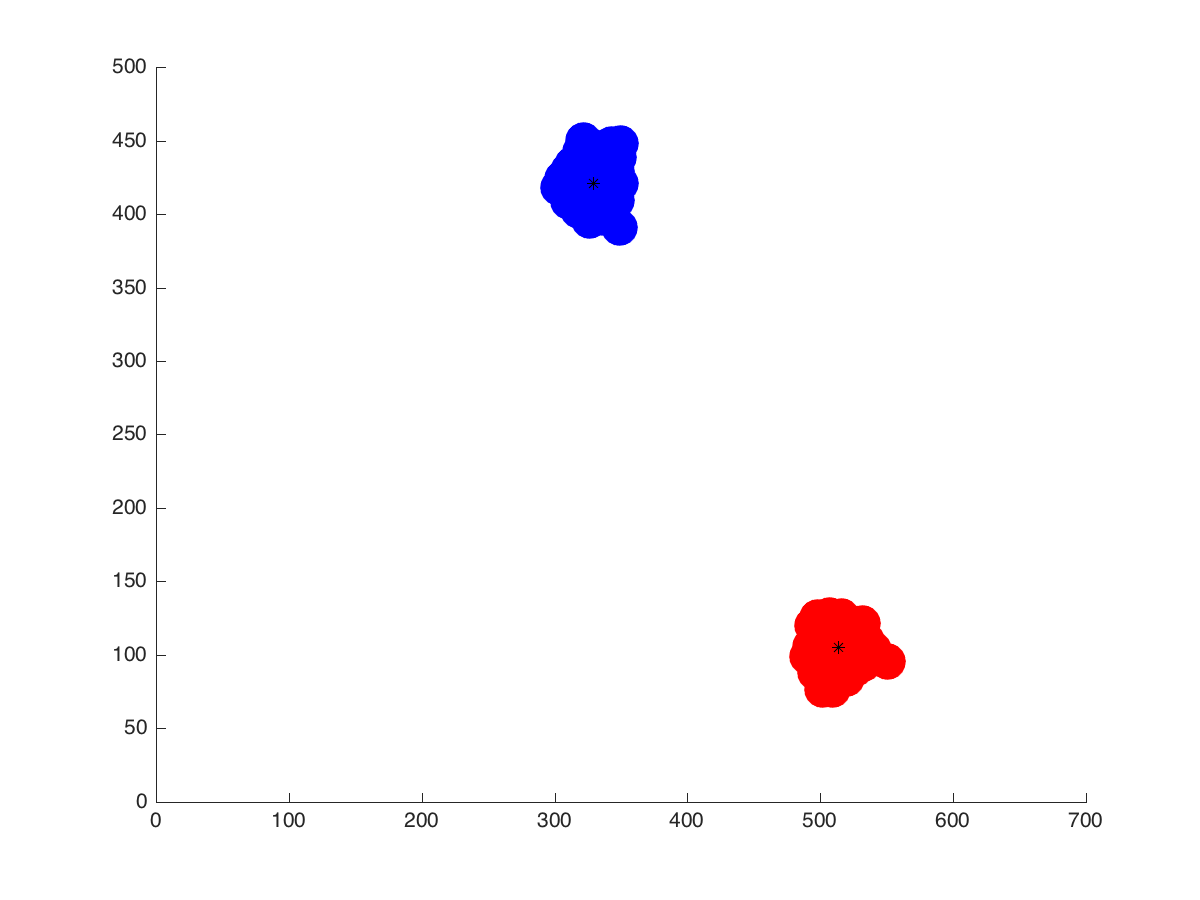
\includegraphics[width=1\textwidth]{figures/Scene.png}
    \captionof{figure}{Scene representation}
    \label{fig:scene}
  \end{minipage}
  \hfill
  \begin{minipage}[b]{0.60\textwidth}
    \centering
    \begin{tabular}{cc}\hline
        \textbf{Reward} & \textbf{Action Condition}\\ \hline
        
        \textcolor{ForestGreen}{+30} & Grasp \textbf{\textcolor{red}{red}} item \\
        \textcolor{ForestGreen}{+10} & Grasp \textbf{\textcolor{blue}{blue}} item \\
        \textcolor{OrangeRed}{-100} & Miss item grasp by 11px \\
        \textcolor{OrangeRed}{-1} & Per item not attempted \\
        \hline
        \\
        
      \end{tabular}
      \captionof{table}{Rewords for the agent's training}
      \label{table:rewards}
    \end{minipage}

\begin{figure}[h]
	\centering
	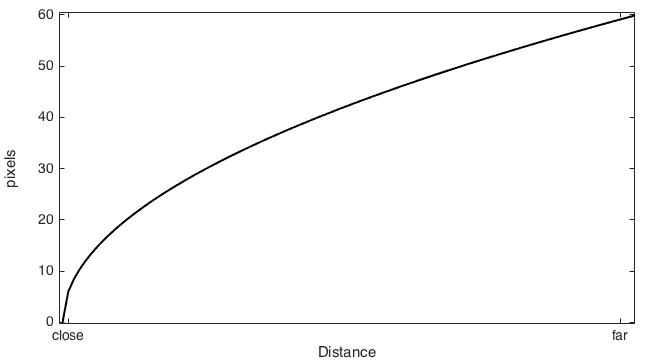
\includegraphics[width=0.7\textwidth]{figures/Noise.png}
	\caption{Function of noisy displacement as distance increases}
	\label{fig:noise}
\end{figure}

The scenario forces a competitive decision between which item to give focus to. 
The world state is represented by the position of the two items, however, due to noisy perception, the true location must be estimated.
As there is time only to accurately observe a single item, subjects must decide which of the two is more optimal to gain certainty about. 
The scenario therefore constrains subjects to perform in a situation requiring optimal gaze control. 

Optimal behaviour would dictate subjects to focus on the item which renders the highest reward. 
Performing in the task requires learning both an optimal gaze strategy, but also the adequate level of certainty needed to execute successful grasping.  
Our model learns optimal behaviour through reinforcement learning by internally representing the world's state of uncertainty. 


\section{Representing Uncertainty}
In order to support robust decision making, one must represent the amount of uncertainty present in the world. 
That is, given prior information received thus far, how credible is the posterior belief about an item's position. 
As mentioned previously, nature may employ a form of Bayesian inference for this process.
Our model mimics inference and represents uncertainty through the use of particle filters. 

Particle filters are a technique used in robotics to estimate the state of a system given noisy sensory hardware.
Through it's operation, the filter emulates Bayesian inference.   
For example, given the current set of information, particles cluster around the approximate location of an observed item.
As new information becomes available, the particles gather tighter around the item's location.
This indicates both a decrease in uncertainty and a better approximation of position. 
The process is best described in figure \ref{fig:uncertainty}, in how uncertainty gradually decreases to eventually represent the likely state of the world. 

\begin{figure}[h]
	\centering
	\includegraphics[width=0.7\textwidth]{figures/uncertainty.png}
	\caption{Visual information decreasing uncertainty}
	\label{fig:uncertainty}
\end{figure}

We denote the spread of particles for each item to be the agent's belief state. 

\section{Learning From Feedback}
The learning strategy follows the methods described in Rashej Rao's decision making under uncertainty \cite{rashejrao}.
Our agent is trained over 8000 trials using reinforcement learning and an actor critic model (fig. \ref{fig:actor-critic}). 
\begin{figure}[h]
	\centering
	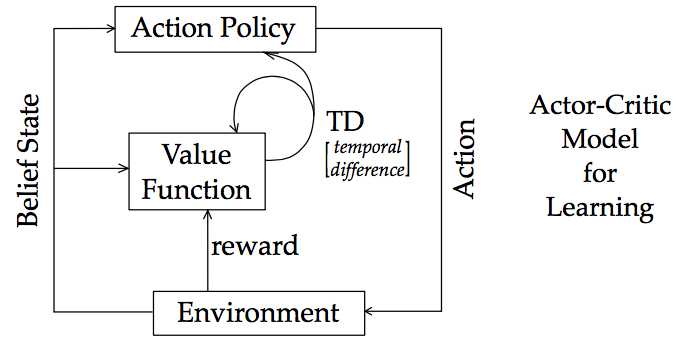
\includegraphics[width=0.7\textwidth]{figures/actorcritic.png}
	\caption{}
	\label{fig:actor-critic}
\end{figure} 

The value function of an actor critic model returns the expected reward for the current belief state.
For example, in complete uncertainty, the expected reward is low regardless of what actions can be taken.
When uncertainty is low however, the chances of reward are higher even if non-optimal decisions are made.  
The mean location of particles in a filter is taken as the estimated item location.
If the particle spread is large, in uncertainty, the item's location is unlikely to be correct. 

The difference over time steps in a value function is used to train a corresponding action policy.
There are two policies the agent must learn: when to grasp and which item to gaze at.
Therefore, there are two value functions as well. 
The action policy returns the probability an action should have, given the current belief state.
For grasping, the policy returns the probability of attempting to grasp an item given its uncertainty spread.
For gazing, the policy returns the probability of focusing at one item or the other given their respective value and level of uncertainty.

Each pair of value function and action policy are learned using radial basis function(RBF) networks (fig. \ref{fig:rbf}).
The components of the RBF networks are:
\begin{list}{}{}
 \item $\pmb{b_t}$ - is the belief state, represented by an item's particle filter spread (as eigenvalues) and the item's reward. 

 \item $\pmb{g_i}$ - is a non-linear Gaussian kernel function ($\sigma=0.25$).
   The kernel centers($\mu$), also known as belief points, act as a receptive field for the belief state.

 \item $\pmb{v_i}$ \& $\pmb{w_i}$ - output layer weights, similar to a feed forward network

 \item $\pmb{V(b_t)}= \Sigma[v_i * g_i(b_t)]$ - value function

 \item $\pmb{A_j(b_t)}= \Sigma[w_{ji} * g_i(b_t)]$ - action value.
   Although network output is probability calculated as $P_{action} = softmax(A_1(b_t),A_2(b_t))$; 
   Where \textbf{softmax} is a normalised exponential function.
\end{list}

\begin{figure}[h]
	\centering
	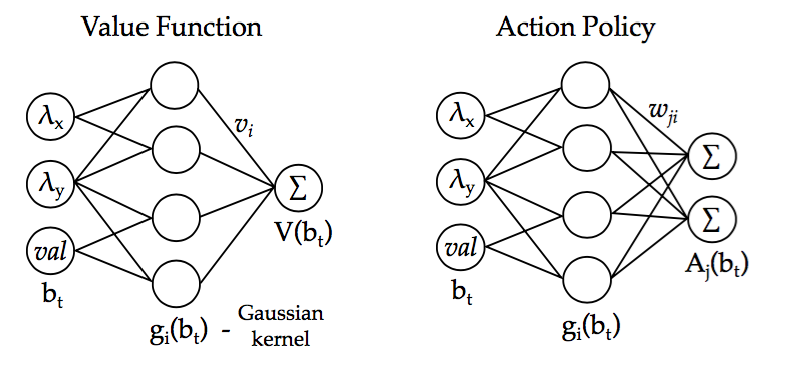
\includegraphics[width=0.7\textwidth]{figures/rbf.png}
	\caption{}
	\label{fig:rbf}
\end{figure} 

\begin{figure}[h]
	\centering
	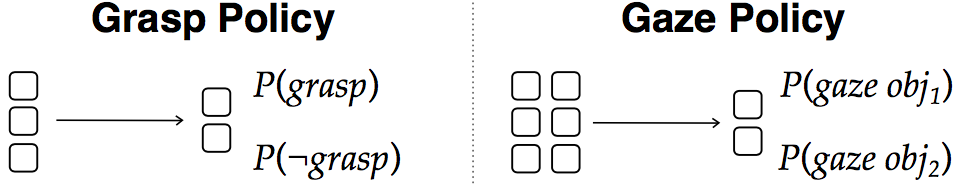
\includegraphics[width=0.7\textwidth]{figures/inputoutput.png}
	\caption{Grasping takes the X-Y coordinate eigenvalues and the value of a single item. Gazing takes both item eigenvalues and reward values.}
	\label{fig:inout}
\end{figure}

Grasp learning requires only a single item's uncertainty and value, whilst gazing requires both. 
This is due to grasping only relying on a single item's uncertainty spread to succeed.
Gazing however brings a competitive decision between the low and high value items.
Gazing therefore requires knowledge of both items for a decision to be made (fig. \ref{fig:inout}). 

Grasp learning is trained in an online fashion using reinforcement learning.
However, the Gaussian layer of the network is determined prior to training through k-means clustering across a randomly generated belief state values.
Our architecture consists of 60 units for the Gaussian layer. 
Reinforcement learning is then used in training the output layer weights.
The grasp decision is learned from the reward generated by the environment and follows the update equations : 

\begin{list}{}{}
  \item \textbf{reward = received from environment}; see table \ref{table:rewards}
  \item $\pmb{TD = reward + V(b_{t+1}) - V(b_t)}$; temporal difference
  \item $\pmb{v_i = v_i + 0.001 * TD * g_i(b_t)}$; value function weights
  \item $\pmb{w_{ji} = w_{ji}+ 0.0005 * TD * g_i(b_t)}$; action policy weights
\end{list}  

Optimal gaze is trained in a similar manner. 
The Gaussian layer consists of 180 kernel centers that are distributed through k-means clustering. 
However, in training the output layer reward is taken as the sum of expected improvement over grasping reward. 
Therefore, environment rewards do not directly feed into optimal gaze learning. 
The model would not result in exclusively focusing on the item rendering highest reward.
Instead, gaze actions depend on grasp learning and the expected reward of such actions.
More exactly, gaze learning depends on the expected improvement in grasp reward for both items.
This improvement is generated by a decrease in uncertainty for both items. 

In gaze learning, the action policy returns the probability of gazing at one object or the other. In order to achieve optimal gaze, we assume that gaze reward should be the sum of expected improvement over grasping reward. Since the value of grasping increases at the same time as the probability of executing a grasp action, we can use grasping probabilities instead of actual reward value. The advantage of this approach is that probabilities will always be within the range of [0,1] and would not be affected by changes in reward value from the environment. 
\begin{list}{}{}
  \item $\pmb{reward = \sum_{item}[P_{grasp}(b_{t+1}) -  P_{grasp}(b_t)] }$; 
  \item $\pmb{TD = reward - V(b_t)}$; temporal difference
  \item $\pmb{ v_i = v_i + 0.8 * TD * g_i(b_t)}$; value function weights
  \item $\pmb{w_{ji} = w_{ji}+ 0.4 * TD * g_i(b_t)}$; action policy weights
\end{list}  

In learning either grasp or gaze, the belief points of each neural network can also be moved in the direction favoring gradient ascent\cite{rashejrao}. The approach was tested but did not render noticeable improvements. Learning success depends highly on the initial distribution of belief points. Future work should consider alternative strategies for spreading belief points. For example, considering k-means clustering over possible values of the belief space, as opposed to randomly generated values.

\pagebreak

\section{Results}
Both grasping and gazing were successfully learned. In order to establish a baseline for performance, reward was recorded for grasping whilst randomly gazing. 
Figure \ref{fig:results} shows the success of the learning technique and a large difference between an optimal gaze strategy vs random gazing. The graph is the result of learning using all the parameters previously described. The faded blue and red areas represent the standard error over 100 training runs.
%
\begin{figure}[h]
	\centering
	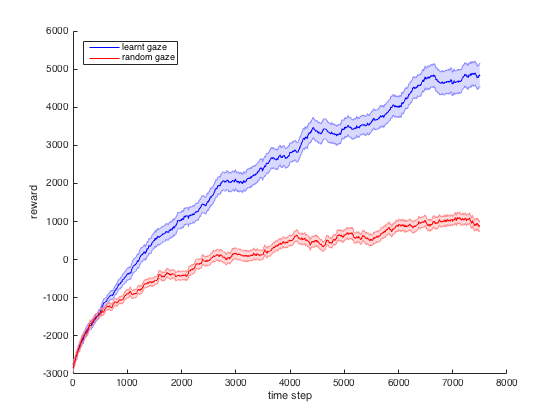
\includegraphics[width=0.7\textwidth]{figures/results.png}
	\caption{}
	\label{fig:results}
\end{figure}

\subsection{Additional Results}
We also explore a scenario where the agent is allowed to make as many visual fixations as wanted before having to make grasp decisions. The agent is allowed to grasp either object or both, although he may do so when becoming completely certain about object positions. We incentivise grasping by penalising the agent for each time step where it chooses to gaze without grasping.

Figure \ref{fig:resultsTimless} shows that optimal gaze has a very small impact on overall task performance. However, when looking on the number of fixations, optimal gaze tends to fixate noticeably fewer times than random gaze (fig. \ref{fig:gazeCount}). Both figures contain the average and standard error collected over 20 training runs whilst using a size 500 moving window sum.

\begin{figure}[h]
	\centering
	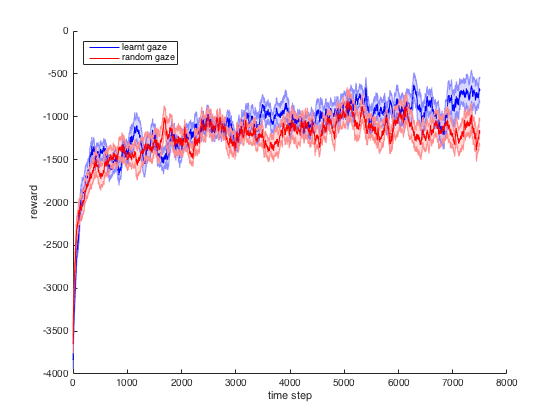
\includegraphics[width=0.7\textwidth]{figures/resultsTimeless.png}
	\caption{Task performance for as many fixations as needed}
	\label{fig:resultsTimless}
\end{figure}


\begin{figure}[!h]
	\centering
	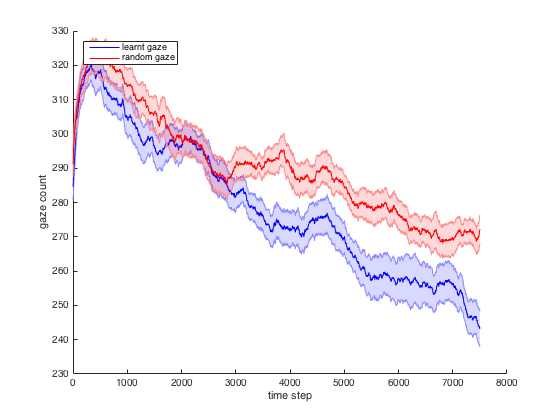
\includegraphics[width=0.7\textwidth]{figures/gazeCount.png}
	\caption{Number of fixations before grasp (moving window sum)}
	\label{fig:gazeCount}
\end{figure}

\pagebreak

\begin{thebibliography}{9}
\bibitem{nunezvalera}
Nunez-Varela, J. and Wyatt, J. L. (2013) ‘Models of gaze control for manipulation tasks’, ACM Transactions on Applied Perception, 10(4), pp. 1-22. doi: 10.1145/2536764.2536767.

\bibitem{rashejrao}
Rao, R. P. N. (2010). Decision making under uncertainty: A neural model based on partially observable Markov decision processes. Frontiers in Computational Neuroscience, 4, . doi:10.3389/fncom.2010.00146

\end{thebibliography}

\end{document}
